% Workflow diagram for the SurveyNCD papers. Build: pdflatex fig_workflow.tex
\documentclass[tikz,border=4pt]{standalone}
\usepackage[scaled]{helvet}\renewcommand{\familydefault}{\sfdefault}
\usetikzlibrary{positioning,arrows.meta}
\definecolor{blue}{HTML}{2A78D6}\definecolor{ink}{HTML}{52514E}\definecolor{fill}{HTML}{EEF4FC}
\definecolor{grey}{HTML}{F2F1EE}
\tikzset{
  box/.style={draw=blue, fill=fill, rounded corners=3pt, line width=0.7pt,
              align=center, minimum height=12mm, text width=33mm, font=\footnotesize},
  ext/.style={draw=ink, fill=grey, rounded corners=3pt, dashed, line width=0.6pt,
              align=center, minimum height=12mm, text width=33mm, font=\footnotesize},
  arr/.style={-{Stealth[length=2.2mm]}, line width=0.7pt, draw=ink}
}
\begin{document}
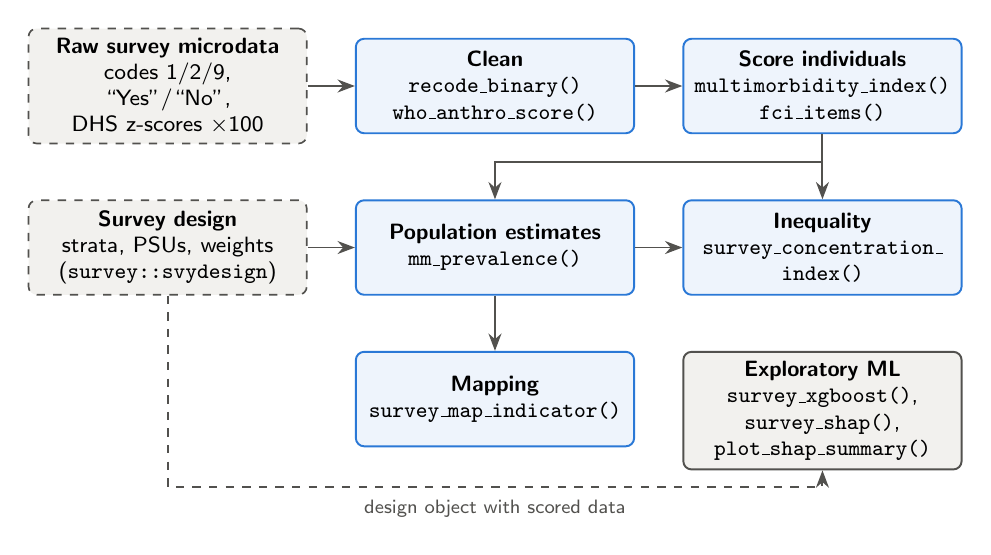
\begin{tikzpicture}[node distance=7mm and 6mm]
\node[ext] (raw) {\textbf{Raw survey microdata}\\ codes 1/2/9, ``Yes''/``No'',\\ DHS z-scores $\times$100};
\node[box, right=of raw] (clean) {\textbf{Clean}\\ \texttt{recode\_binary()}\\ \texttt{who\_anthro\_score()}};
\node[box, right=of clean] (score) {\textbf{Score individuals}\\ \texttt{multimorbidity\_index()}\\ \texttt{fci\_items()}};
\node[ext, below=of raw] (design) {\textbf{Survey design}\\ strata, PSUs, weights\\ (\texttt{survey::svydesign})};
\node[box, right=of design] (prev) {\textbf{Population estimates}\\ \texttt{mm\_prevalence()}};
\node[box, right=of prev] (ineq) {\textbf{Inequality}\\ \texttt{survey\_concentration\_}\\ \texttt{index()}};
\node[box, below=of prev] (map) {\textbf{Mapping}\\ \texttt{survey\_map\_indicator()}};
\node[box, draw=ink, fill=grey, below=of ineq] (ml) {\textbf{Exploratory ML}\\ \texttt{survey\_xgboost()}, \texttt{survey\_shap()},\\ \texttt{plot\_shap\_summary()}};
\draw[arr] (raw) -- (clean); \draw[arr] (clean) -- (score);
\draw[arr] (score.south) |- ++(0,-3.5mm) -| (prev.north);
\draw[arr] (score.south) -- (ineq.north);
\draw[arr] (design) -- (prev); \draw[arr] (prev) -- (ineq);
\draw[arr] (prev) -- (map);
\draw[arr, dashed] (design.south) |- ([yshift=-5mm]map.south) -| (ml.south);
\node[font=\scriptsize, text=ink, anchor=north] at ([yshift=-5.5mm]map.south) {design object with scored data};
\end{tikzpicture}
\end{document}
